\documentclass[10pt,xcolor={x11names}]{beamer}

\usetheme[numbering=fraction,block=fill]{metropolis}
\usecolortheme{seahorse}
\setbeamertemplate{blocks}[rounded]

\usepackage{kmath}
% Tikz
\usetikzlibrary{calc}
\usetikzlibrary{mindmap,trees,shapes,arrows,backgrounds,topaths}
\usetikzlibrary{decorations.pathmorphing, shapes.geometric}

% Text
\usepackage{enumitem}
\usepackage{ulem}
\usepackage{pifont}

% Maths
\usepackage{amsmath}
\usepackage{amsfonts}
\usepackage{amsthm}
\usepackage{amsopn}

% Plots
\usepackage{pgfplots}
\usepgfplotslibrary{groupplots}

% Tables
\usepackage{booktabs}
\usepackage{array}
\newcolumntype{L}{>$l<$}
\arraycolsep=1.4pt
\setlength{\tabcolsep}{3pt}

% Algos
\usepackage[ruled]{algorithm2e}

% Pgfplot
\pgfplotsset{
    legend image code/.code={
        \draw[mark repeat=2,mark phase=2] plot coordinates {
            (0cm,0cm)
            (0.25cm,0cm)
            (0.25cm,0cm)
        };
    }
}
% Objective values and functions
\newcommand{\pobj}{p}
\newcommand{\robj}{r}
\newcommand{\dobj}{d}

% Variables
\newcommand{\pvletter}{x}
\newcommand{\wvletter}{w}
\newcommand{\dvletter}{u}
\newcommand{\vvletter}{v}
\newcommand{\bvletter}{z}
\newcommand{\pv}{\mathbf{\pvletter}}
\newcommand{\wv}{\mathbf{\wvletter}}
\newcommand{\dv}{\mathbf{\dvletter}}
\newcommand{\vv}{\mathbf{\vvletter}}
\newcommand{\bv}{\mathbf{\bvletter}}
\newcommand{\pvi}[1]{\pvletter_{#1}}
\newcommand{\wvi}[1]{\wvletter_{#1}}
\newcommand{\dvi}[1]{\dvletter_{#1}}
\newcommand{\vvi}[1]{\vvletter_{#1}}
\newcommand{\bvi}[1]{\bvletter_{#1}}

% Problem data
\newcommand{\pdim}{n}
\newcommand{\ddim}{m}
\newcommand{\dic}{\mathbf{A}}
\newcommand{\dici}[1]{\mathbf{a}_{#1}}
\newcommand{\dicii}[1]{a_{#1}}
\newcommand{\obs}{\mathbf{y}}
\newcommand{\obsi}[1]{y_{#1}}
\newcommand{\reg}{\lambda}
\newcommand{\groundtruth}{\pv^{\dagger}}
\newcommand{\lfunc}{f}
\newcommand{\pfunc}{h}
\newcommand{\rfunc}{g}
\newcommand{\dfunc}{D}
\newcommand{\relaxrfunc}{\tilde{g}}
\newcommand{\relaxpfunc}{\tilde{h}}
\newcommand{\bigM}{M}
\newcommand{\regtwo}{\alpha}
\newcommand{\rslope}{\tau}
\newcommand{\rlimit}{\mu}
\newcommand{\noise}{\boldsymbol{\epsilon}}

% Indices
\newcommand{\idxentry}{i}

% BnB
\newcommand{\pset}{\mathcal{X}}
\newcommand{\setidx}{\mathcal{S}}
\newcommand{\setzero}{\setidx_0}
\newcommand{\setone}{\setidx_1}
\newcommand{\setnone}{\setidx_\bullet}
\newcommand{\nodeSymb}{\nu}
\newcommand{\node}[1]{#1^{\nodeSymb}}

% Screening
\newcommand{\saferegion}{\mathcal{R}}
\newcommand{\safesphere}{\mathcal{S}}
\newcommand{\spherecenter}{\mathbf{c}}
\newcommand{\sphereradius}{r}

% Peeling
\newcommand{\bigL}{\boldsymbol{\alpha}}
\newcommand{\bigU}{\boldsymbol{\beta}}
\newcommand{\bigLi}[1]{\alpha_{#1}}
\newcommand{\bigUi}[1]{\beta_{#1}}

% Math operators
\DeclareMathOperator{\argmax}{argmax}
\DeclareMathOperator{\argmin}{argmin}
\DeclareMathOperator{\biconjugate}{biconj}
\DeclareMathOperator{\card}{card}
\DeclareMathOperator{\complset}{cmpl}
\DeclareMathOperator{\convex}{cvx}
\DeclareMathOperator{\diam}{diam}
\DeclareMathOperator{\dom}{dom}
\DeclareMathOperator{\interior}{int}
\DeclareMathOperator{\prox}{prox}
\DeclareMathOperator{\rank}{rank}
\DeclareMathOperator{\sign}{sign}


% Math misc
\newcommand{\1}{\mathbf{1}}
\newcommand{\0}{\mathbf{0}}
\newcommand{\abs}[1]{|#1|}
\newcommand{\biconj}[1]{#1^{**}}
\newcommand{\bigO}{\mathcal{O}}
\newcommand{\conj}[1]{#1^{*}}
\newcommand{\icvx}{\eta}
\newcommand{\intervint}[2]{[#1,#2]}
\newcommand{\iter}[2]{#1^{#2}}
\newcommand{\norm}[2]{\|#1\|_#2}
\newcommand{\opt}[1]{#1^{\star}}
\newcommand{\pospart}[1]{[#1]_+}
\newcommand{\separable}[2]{#1_{#2}}
\newcommand{\subdiff}{\partial}
\newcommand{\transp}[1]{#1^{\mathrm{T}}}

% Edition macros
\newcommand{\AddTodo}[1]{\textcolor{red}{[#1]}}

% Colors
\definecolor{Brown}{HTML}{EB811B}
\definecolor{Teal}{HTML}{137D91}
\definecolor{Red}{HTML}{C8412F}
\definecolor{Green}{HTML}{14B03D}

% Beamer elements
\newcommand{\emphcolor}[2]{{\color{#1}#2}}
\newenvironment<>{blockcolor}[2]{%
  \setbeamercolor{block title}{fg=#1,bg=#1!15}%
  \setbeamercolor{block body}{fg=#1,bg=#1!15}%
  \begin{block}#3{\centering#2\par}}{\end{block}}

\title{\large{Discrete optimization methods for sparse problems}}
\date{Inria, Centre de l'Université de Rennes, France}
\author{\textbf{Théo Guyard}}
\institute{Journée Doctorant·e·s Rennais·e·s en Statistique \\ 18th of March, 2024 \\ Rennes, France}


\begin{document}

\maketitle

\section{Sparse problems}

\begin{frame}{Two goals, one problem}
  \begin{tikzpicture}[remember picture,overlay]
    \draw [ultra thick,<->] ($(current page.north)+(-2.2,-0.32\textheight)$) -- ($(current page.north)+(2.2,-0.32\textheight)$) node (arrow) [midway] {};
    \node at ($(arrow.north)+(0,0.1)$) {\textbf{Sparse problems}};
    \node [text width=0.3\textwidth] at ($(current page.north)+(-4,-0.3\textheight)$) (obs) {
        \begin{blockcolor}{Brown}{}
            \centering
            \textbf{Optimize a function}
        \end{blockcolor}
    };
    \node [text width=.3\textwidth] at ($(current page.north)+(4,-0.3\textheight)$) (dic) {
      \begin{blockcolor}{Brown}{}
            \centering
            \textbf{Sparse solution}
        \end{blockcolor}
    };
    %
    %
    %
    \node at ($(current page.north)+(-2.5,-0.65\textheight)$) (sp) {};
    \node at (sp) {Signal processing};
    \draw ($(sp)+(0,1)$) node {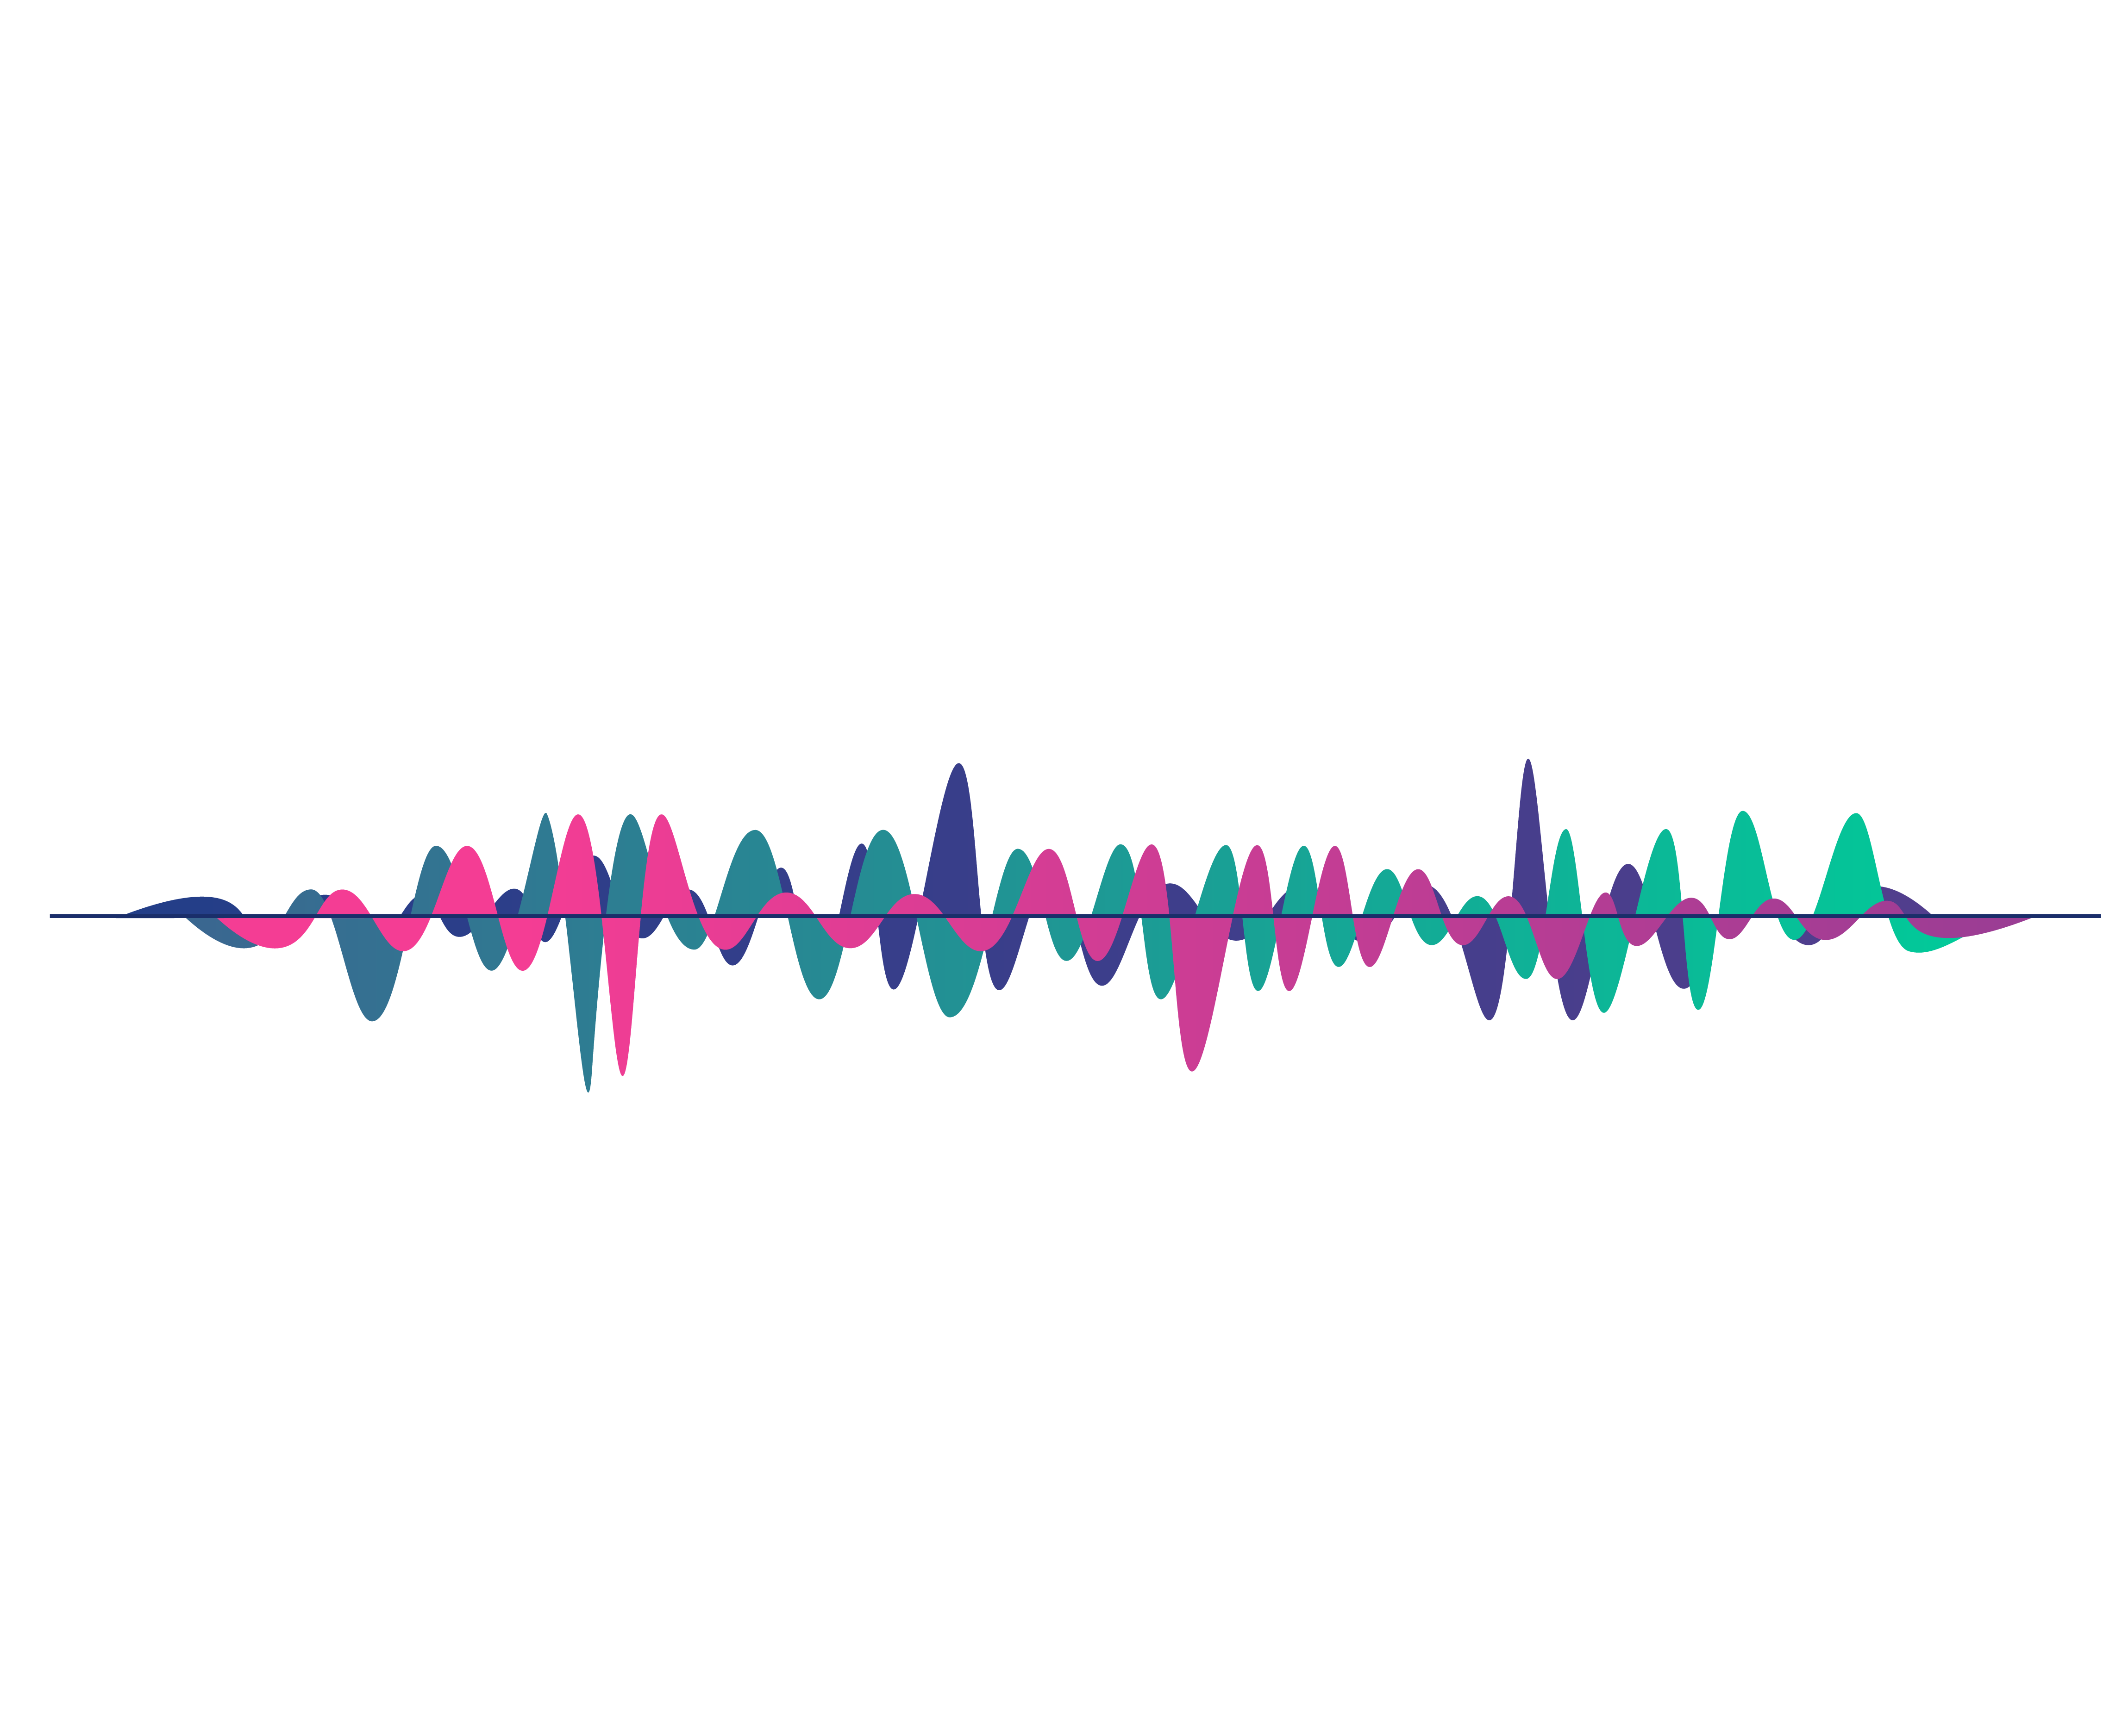
\includegraphics[width=4cm]{imgs/signal-processing.png}};
    %
    %
    %
    \node at ($(current page.north)+(2.5,-0.65\textheight)$) (ml) {};
    \node at (ml) {Machine learning};
    \draw ($(ml)+(0,1)$) node {
\includegraphics[width=2cm]{imgs/machine-learning.png}};
    %
    %
    %
    \node at ($(current page.north)+(-2.5,-0.95\textheight)$) (nd) {};
    \node at (nd) {High-dim. statistics};
    \draw ($(nd)+(0,1.25)$) node {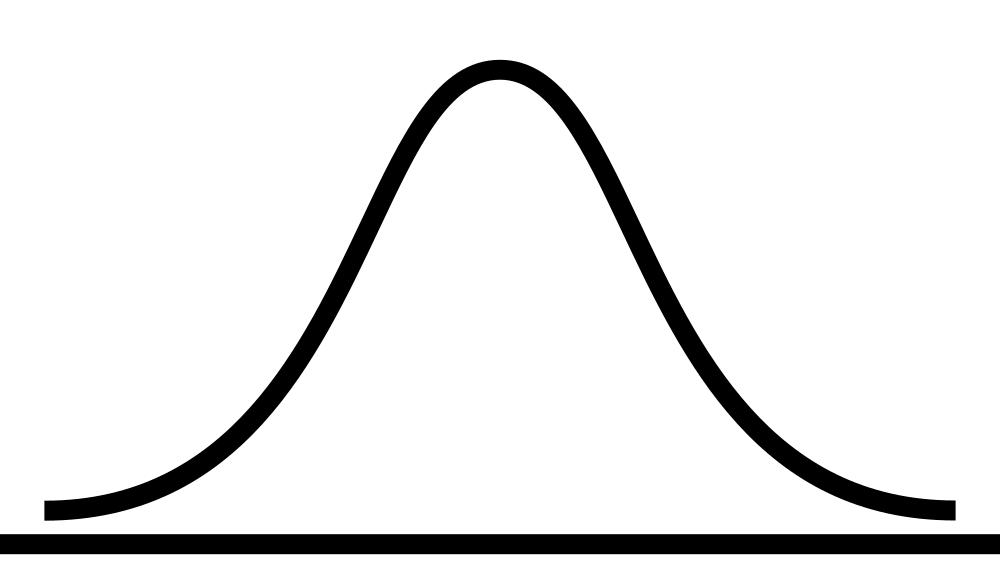
\includegraphics[width=2cm]{imgs/stat.png}};
    %
    %
    %
    \node at ($(current page.north)+(2.5,-0.95\textheight)$) (others) {};
    \node at (others) {And many others};
    \draw ($(others)+(0,1.25)$) node {
\includegraphics[width=1.25cm]{imgs/nerd_face.png}};
  \end{tikzpicture}
\end{frame}

\begin{frame}{Example}
    \begin{tikzpicture}[remember picture,overlay]
        \onslide<+-> {
            \node [text width=0.45\textwidth] at ($(current page.north)+(-3,-0.3\textheight)$) (glm) {
                \begin{blockcolor}{black}{}
                    \centering
                    \textbf{Sparse GLM}
                \end{blockcolor}
            };
            \node [align=center,text width=0.45\textwidth] at ($(glm)+(0,-0.125\textheight)$) (glm-data) {\emphcolor{black}{$ \, $ Features $\dic \in \kR^{\ddim\times\pdim}$ \\ Targets $\obs \in \kR^{\ddim}$}};
            \node [align=center,text width=0.45\textwidth] at ($(glm-data)+(0,-0.2\textheight)$) (glm-prob) {
                \begin{blockcolor}{black}{}
                    \centering
                    $\max_{\pv} \ \mathcal{L}(\dic\pv,\obs)$
                \end{blockcolor}
            };
            \draw[ultra thick,->] (glm-data.south) -- ($(glm-prob.north)+(0,-0.3)$);
            \node [align=center,text width=0.45\textwidth] at ($(glm-prob)+(0,-0.1\textheight)$) (glm-cond) {No unique solution when \emphcolor{Brown}{$\ddim \ll \pdim$}};
            \node [align=center,text width=0.45\textwidth] at ($(glm-cond)+(0,-0.175\textheight)$) (glm-prob-sparse) {
                \begin{blockcolor}{Brown}{}
                    \centering
                    $\max_{\pv} \ \mathcal{L}(\dic\pv,\obs) \ \text{with} \ \pv \ \text{sparse}$
                \end{blockcolor}
            };
            \draw[ultra thick,->] (glm-cond.south) -- ($(glm-prob-sparse.north)+(0,-0.3)$);
        }
        \onslide<+-> {
            \node [text width=0.45\textwidth] at ($(current page.north)+(3,-0.3\textheight)$) (glm) {
                \begin{blockcolor}{black}{}
                    \centering
                    \textbf{Sparse PCA}
                \end{blockcolor}
            };
            \node [align=center,text width=0.45\textwidth] at ($(glm)+(0,-0.125\textheight)$) (glm-data) {\emphcolor{black}{$ \, $ Features $\dic \in \kR^{\ddim\times\pdim}$ \\ Covariance $\Sigma = \transp{\dic}\dic$}};
            \node [align=center,text width=0.45\textwidth] at ($(glm-data)+(0,-0.2\textheight)$) (glm-prob) {
                \begin{blockcolor}{black}{}
                    \centering
                    $\max_{\norm{\pv}{2}=1} \ \transp{\pv}\Sigma\pv$
                \end{blockcolor}
            };
            \draw[ultra thick,->] (glm-data.south) -- ($(glm-prob.north)+(0,-0.3)$);
            \node [align=center,text width=0.45\textwidth] at ($(glm-prob)+(0,-0.1\textheight)$) (glm-cond) {Not relevant when \emphcolor{Brown}{$\ddim \ll \pdim$}};
            \node [align=center,text width=0.45\textwidth] at ($(glm-cond)+(0,-0.175\textheight)$) (glm-prob-sparse) {
                \begin{blockcolor}{Brown}{}
                    \centering
                    $\max_{\norm{\pv}{2}=1} \ \transp{\pv}\Sigma\pv \ \text{with} \ \pv \ \text{sparse}$
                \end{blockcolor}
            };
            \draw[ultra thick,->] (glm-cond.south) -- ($(glm-prob-sparse.north)+(0,-0.3)$);
        }
    \end{tikzpicture}
\end{frame}

\begin{frame}{Example}
    \begin{tikzpicture}[remember picture,overlay]
        \onslide<+-> {
            \node at ($(current page.north)+(0,-0.35\textheight)$) {
                \begin{tabular}{cccccc}
                    \multicolumn{6}{c}{\textbf{Heart disease dataset (LIBSVM)}} \\
                    \toprule
                    Age & Sex & Cholesterol & Blood pressure & ... & \textbf{Disease} \\
                    \midrule
                    31 & M & 50.3 mg/dl  & 95 mm/hg & ... & \textbf{No} \\
                    35 & F & 54.9 mg/dl & 98 mm/hg & ... & \textbf{Yes} \\
                    42 & F & 49.8 mg/dl & 92 mm/hg & ... & \textbf{Yes} \\
                    37 & M & 59.1 mg/dl & 89 mm/hg & ... & \textbf{No} \\
                    ... & ... & ... & ... & ... & ... \\
                    \bottomrule
                \end{tabular}
            };
        }
        %
        %
        %
        \onslide<+-> {
            \node[align=center,text width=0.2\textwidth] (data) at ($(current page.north)+(-4.5,-0.7\textheight)$) {
                \begin{blockcolor}{black}{}
                    \centering\textbf{Data}
                \end{blockcolor}
            };
            %
            \node[align=center,text width=0.3\textwidth] (logreg) at ($(current page.north)+(0,-0.7\textheight)$) {
                \begin{blockcolor}{black}{}
                    \centering\textbf{Logistic regression}
                \end{blockcolor}
            };
            \draw[ultra thick,->] ($(data.east)+(0.1,-0.2)$) -- ($(logreg.west)+(-0.1,-0.2)$);
            %
            \node[align=center,text width=0.2\textwidth] (estimator) at ($(current page.north)+(4.5,-0.7\textheight)$) {
                \begin{blockcolor}{black}{}
                    \centering\textbf{Estimator $\pv$}
                \end{blockcolor}
            };
            \draw[ultra thick,->] ($(logreg.east)+(0.1,-0.2)$) -- ($(estimator.west)+(-0.1,-0.2)$);
        }
        %
        %
        %
        \onslide<+-> {
            \draw[ultra thick,<-,Brown] ($(estimator.south)+(-0.75,-0)$) .. controls ($(estimator.south)+(-1,-0.5)$) .. ($(estimator.south)+(-1,-1)$) node[below,align=center,text width=0.6\textwidth] {Involves all the features \\ Explainability and robustness issues};
        }
        %
        %
        %
        \onslide<+-> {
            \draw[ultra thick,<-,Brown] ($(logreg.south)+(-1.75,-0)$) .. controls ($(logreg.south)+(-2,-0.5)$) .. ($(logreg.south)+(-2,-1)$) node[below,align=center,text width=0.6\textwidth] {Force the use of only few \\ features via sparsity in $\pv$};
        }
    \end{tikzpicture}
\end{frame}

\begin{frame}{Objective, constraint or both ?}
    \begin{tikzpicture}[remember picture,overlay]
        \onslide<+-> {
            \draw [ultra thick,<->] ($(current page.north)+(-2.2,-0.32\textheight)$) -- ($(current page.north)+(2.2,-0.32\textheight)$) node (arrow) [midway] {};
            \node at ($(arrow.north)+(0,0.1)$) {\textbf{Sparse optimization}};
            \node [text width=0.3\textwidth] at ($(current page.north)+(-4,-0.3\textheight)$) (obs) {
                \begin{blockcolor}{Brown}{}
                    \centering
                    \textbf{Optimize a function}
                \end{blockcolor}
            };
            \node at ($(current page.north)+(-4,-0.4\textheight)$) {\emphcolor{Brown}{Loss function $\lossfunc(\pv)$}};
            \node [text width=.3\textwidth] at ($(current page.north)+(4,-0.3\textheight)$) {
            \begin{blockcolor}{Brown}{}
                    \centering
                    \textbf{Sparse solution}
                \end{blockcolor}
            };
            \node at ($(current page.north)+(4,-0.4\textheight)$) {\emphcolor{Brown}{Counting function $\norm{\pv}{0}$}};
        }
        %
        %
        %
        \onslide<+-> {
            \node [text width=0.4\textwidth] at ($(current page.north)+(-3,-0.6\textheight)$) (problem-constraint) {
                \begin{blockcolor}{black}{Constrainted version}
                    \centering
                    $\min_{\pv} \lossfunc(\pv) \ \text{s.t.} \ \norm{\pv}{0} \leq \kappa$
                \end{blockcolor}
            };
            %
            %
            %
            \node [text width=0.4\textwidth] at ($(current page.north)+(3,-0.6\textheight)$) (problem-constraint) {
                \begin{blockcolor}{black}{Minimized version}
                    \centering
                    $\min_{\pv}  \norm{\pv}{0} \ \text{s.t.} \ \lossfunc(\pv) \leq \epsilon$
                \end{blockcolor}
            };
            %
            %
            %
            \node [text width=0.4\textwidth] at ($(current page.north)+(0,-0.85\textheight)$) (problem-constraint) {
                \begin{blockcolor}{black}{Penalized version}
                    \centering
                    $\min_{\pv} \lossfunc(\pv) + \reg \norm{\pv}{0}$
                \end{blockcolor}
            };
        }
    \end{tikzpicture}
\end{frame}

\begin{frame}{A bit of history}
    \begin{tikzpicture}[remember picture,overlay]
        \draw [ultra thick,->] ($(current page.north)+(-6,-0.3\textheight)$) -- ($(current page.north)+(6,-0.3\textheight)$) node (arrow) [midway] {};
        %
        %
        %
        \onslide<+-> {
            \node (date1) at ($(current page.north)+(-5,-0.3\textheight)$) {};
            \draw [ultra thick,-] ($(date1)+(0,-0.02\textheight)$) -- ($(date1)+(0,0.02\textheight)$);
            \node at ($(date1)+(0,+0.06\textheight)$)  {\textbf{1990}};
            \node[text width=0.2\textwidth,align=center,font=\small] at ($(date1)+(0,-0.1\textheight)$) {Sparse \\ heuristics};
            \node[text width=0.3\textwidth,align=center,font=\scriptsize] at ($(date1)+(0,-0.22\textheight)$) {\emphcolor{Brown}{MP, OMP, \\ IHT and co.}};
            %
            \node (origin1) at ($(date1)+(0,-0.5\textheight)$) {};
            \node (point1) at ($(date1)+(-0.45,-0.55\textheight)$) {$\pv^{1}$};
            \node (point2) at ($(date1)+(0.025,-0.55\textheight)$) {$\pv^{2}$};
            \node (point3) at ($(date1)+(0.5,-0.55\textheight)$) {$\pv^{3}$};
            \fill[draw,thick,fill=white] ($(origin1)+(-0.5,0)$) circle (0.1);
            \fill[draw,thick,fill=Teal] ($(origin1)+(-0.5,0.3)$) circle (0.1);
            \fill[draw,thick,fill=white] ($(origin1)+(-0.5,0.6)$) circle (0.1);
            \fill[draw,thick,fill=white] ($(origin1)+(-0.5,0.9)$) circle (0.1);
            \fill[draw,thick,fill=white] ($(origin1)+(-0.5,1.2)$) circle (0.1);
            \fill[draw,thick,fill=white] ($(origin1)+(-0.5,1.5)$) circle (0.1);
            \fill[draw,fill=white] ($(origin1)+(0,0)$) circle (0.1);
            \fill[draw,thick,fill=Teal] ($(origin1)+(0,0.3)$) circle (0.1);
            \fill[draw,thick,fill=white] ($(origin1)+(0,0.6)$) circle (0.1);
            \fill[draw,thick,fill=Teal] ($(origin1)+(0,0.9)$) circle (0.1);
            \fill[draw,thick,fill=white] ($(origin1)+(0,1.2)$) circle (0.1);
            \fill[draw,thick,fill=white] ($(origin1)+(0,1.5)$) circle (0.1);
            \fill[draw,thick,fill=white] ($(origin1)+(0.5,0)$) circle (0.1);
            \fill[draw,thick,fill=Teal] ($(origin1)+(0.5,0.3)$) circle (0.1);
            \fill[draw,thick,fill=white] ($(origin1)+(0.5,0.6)$) circle (0.1);
            \fill[draw,thick,fill=Teal] ($(origin1)+(0.5,0.9)$) circle (0.1);
            \fill[draw,thick,fill=Teal] ($(origin1)+(0.5,1.2)$) circle (0.1);
            \fill[draw,thick,fill=white] ($(origin1)+(0.5,1.5)$) circle (0.1);
        }
        %
        %
        %
        \onslide<+-> {
            \node (date2) at ($(current page.north)+(-2.5,-0.3\textheight)$) {};
            \draw [ultra thick,-] ($(date2)+(0,-0.02\textheight)$) -- ($(date2)+(0,0.02\textheight)$);
            \node at ($(date2)+(0,+0.06\textheight)$)  {\textbf{2000}};
            \node[text width=0.2\textwidth,align=center,font=\small] at ($(date2)+(0,-0.1\textheight)$) {Formulation \\ with $\ell_0$-norm};
            \node[text width=0.3\textwidth,align=center,font=\scriptsize] at ($(date2)+(0,-0.22\textheight)$) {\emphcolor{Brown}{RIP, NSP, \\ EkR and co.}};
            %
            \node (origin2) at ($(date2)+(0,-0.5\textheight)$) {};
            \node at ($(origin2)+(0,0.12\textheight)$) {Heuristic};
            \node at ($(origin2)+(0,0.02\textheight)$) {$\ell_0$-prob.};
            \node[rotate=90] at ($(origin2)+(0,0.07\textheight)$) {$\equiv$};
        }
        %
        %
        %
        \onslide<+-> {
            \node (date3) at ($(current page.north)+(0,-0.3\textheight)$) {};
            \draw [ultra thick,-] ($(date3)+(0,-0.02\textheight)$) -- ($(date3)+(0,0.02\textheight)$);
            \node at ($(date3)+(0,+0.06\textheight)$)  {\textbf{2005}};
            \node[text width=0.2\textwidth,align=center,font=\small] at ($(date3)+(0,-0.1\textheight)$) {Convex approx. \\ of $\ell_0$-norm};
            \node[text width=0.3\textwidth,align=center,font=\scriptsize] at ($(date3)+(0,-0.22\textheight)$) {\emphcolor{Brown}{Lasso, Elastic-Net \\ and co.}};
            %
            \node (origin3) at ($(date3)+(0,-0.5\textheight)$) {};
            \draw[ultra thick,->] ($(origin3)+(-1,0)$) -- ($(origin3)+(1, 0)$);
            \draw[ultra thick,->] ($(origin3)+(0,0)$) -- ($(origin3)+(0,1.5)$);
            \draw[ultra thick] ($(origin3)+(-0.03,0.2)$) -- ($(origin3)+(0.03,0.2)$);
            \draw[{Arc Barb[arc=130,reversed]}-,Teal,ultra thick] ($(origin3)+(-0.05,0.8)$) -- ($(origin3)+(-1,0.8)$);
            \draw[{Arc Barb[arc=130,reversed]}-,Teal,ultra thick] ($(origin3)+(0.05,0.8)$) -- ($(origin3)+(1,0.8)$);
            \draw[Teal,ultra thick,dashed] (origin3) .. controls ($(origin3)+(-0.5,0.1)$) ..  ($(origin3)+(-1,0.8)$);
            \draw[Teal,ultra thick,dashed] (origin3) .. controls ($(origin3)+(0.5,0.1)$) ..  ($(origin3)+(1,0.8)$);
            \fill[Teal] (origin3) circle (0.1);
        }
        %
        %
        %
        \onslide<+-> {
            \node (date4) at ($(current page.north)+(2.5,-0.3\textheight)$) {};
            \draw [ultra thick,-] ($(date4)+(0,-0.02\textheight)$) -- ($(date4)+(0,0.02\textheight)$);
            \node at ($(date4)+(0,+0.06\textheight)$)  {\textbf{2013}};
            \node[text width=0.22\textwidth,align=center,font=\small] at ($(date4)+(0,-0.1\textheight)$) {Concave approx. \\ of $\ell_0$-norm};
            \node[text width=0.3\textwidth,align=center,font=\scriptsize] at ($(date4)+(0,-0.22\textheight)$) {\emphcolor{Brown}{SCAD, MCP \\ CEL0 and co.}};
            %
            \node (origin4) at ($(date4)+(0,-0.5\textheight)$) {};
            \draw[ultra thick,->] ($(origin4)+(-1,0)$) -- ($(origin4)+(1, 0)$);
            \draw[ultra thick,->] ($(origin4)+(0,0)$) -- ($(origin4)+(0,1.5)$);
            \draw[ultra thick] ($(origin4)+(-0.03,0.2)$) -- ($(origin4)+(0.03,0.2)$);
            \draw[{Arc Barb[arc=130,reversed]}-,Teal,ultra thick] ($(origin4)+(-0.05,0.8)$) -- ($(origin4)+(-1,0.8)$);
            \draw[{Arc Barb[arc=130,reversed]}-,Teal,ultra thick] ($(origin4)+(0.05,0.8)$) -- ($(origin4)+(1,0.8)$);
            \draw[Teal,ultra thick,dashed] (origin4) .. controls ($(origin4)+(-0.5,0.8)$) ..  ($(origin4)+(-1,0.8)$);
            \draw[Teal,ultra thick,dashed] (origin4) .. controls ($(origin4)+(0.5,0.8)$) ..  ($(origin4)+(1,0.8)$);
            \fill[Teal] (origin4) circle (0.1);
        }
        %
        %
        %
        \onslide<+-> {
            \node (date5) at ($(current page.north)+(5,-0.3\textheight)$) {};
            \draw[ultra thick,-] ($(date5)+(0,-0.02\textheight)$) -- ($(date5)+(0,0.02\textheight)$);
            \node at ($(date5)+(0,+0.06\textheight)$)  {\textbf{2016}};
            \node[text width=0.22\textwidth,align=center,font=\small] at ($(date5)+(0,-0.1\textheight)$) {Exact methods \\ for $\ell_0$-problems};
            \node[text width=0.3\textwidth,align=center,font=\scriptsize] at ($(date5)+(0,-0.22\textheight)$) {\emphcolor{Brown}{MIP, BnB \\ CP and co.}};
            %
            \node (origin5) at ($(date5)+(0,-0.5\textheight)$) {};
            \draw[ultra thick,-] ($(origin5)+(0.7,0.9)$) -- ($(origin5)+(0.4,0.0)$);
            \draw[ultra thick,-] ($(origin5)+(0.7,0.7)$) -- ($(origin5)+(0.3,1.5)$);
            \draw[ultra thick,-] ($(origin5)+(0.4,1.5)$) -- ($(origin5)+(-0.7,0.5)$);
            \draw[ultra thick,-] ($(origin5)+(-0.6,0.7)$) -- ($(origin5)+(-0.3,0)$);
            \draw[ultra thick,-] ($(origin5)+(-0.4,0.1)$) -- ($(origin5)+(0.5,0.1)$);
            \draw[fill] ($(origin5)+(0.4,0.5)$) circle (0.05);
            \draw[fill] ($(origin5)+(0.4,0.8)$) circle (0.05);
            \draw[fill] ($(origin5)+(0.4,1.1)$) circle (0.05);
            \draw[fill] ($(origin5)+(0.1,0.2)$) circle (0.05);
            \draw[fill] ($(origin5)+(0.1,0.5)$) circle (0.05);
            \draw[fill] ($(origin5)+(0.1,0.8)$) circle (0.05);
            \draw[fill] ($(origin5)+(0.1,1.1)$) circle (0.05);
            \draw[fill] ($(origin5)+(-0.2,0.2)$) circle (0.05);
            \draw[fill] ($(origin5)+(-0.2,0.5)$) circle (0.05);
            \draw[fill] ($(origin5)+(-0.2,0.8)$) circle (0.05);
        }
    \end{tikzpicture}
\end{frame}

\section{Mixed-Integer Optimization}

\begin{frame}{Handeling the L0-norm with MIO tools}
    \begin{tikzpicture}[remember picture,overlay]
        \onslide<+-> {
            \node[text width=0.4\textwidth] at ($(current page.north)+(0,-0.21\textheight)$) (problem) {
                \begin{blockcolor}{Brown}{Sparse problem}
                    \centering
                    $\min_{\pv} \lossfunc(\pv) + \reg \norm{\pv}{0}$
                \end{blockcolor}
            };
            %
            \node[text width=0.2\textwidth] at ($(current page.north)+(0,-0.45\textheight)$) (solution) {
                \begin{blockcolor}{black}{}
                    \centering
                    \textbf{Solution}
                \end{blockcolor}
            };
            %
            \draw[ultra thick,->] (problem) -- ($(solution)+(0,0.15)$) node[midway,fill=white,draw] {Solver};
        }
        %
        %
        %
        \onslide<+-> {
            \draw[ultra thick,<-] (problem.south east) .. controls ($(problem.south east)+(1,-0.25)$) .. ($(problem.south east)+(1,-0.5)$) node[below,font=\scriptsize,align=center,text width=0.3\textwidth] {$\ell_0$-norm is non-linear, non-convex, non-smooth, NP-hard, ...};
            \node at ($(problem.south east)+(1,-2)$) {
                
\includegraphics[width=15pt]{imgs/dizzy.png}
            };  
        }
        %
        %
        %
        \onslide<+-> {
            \node[text width=0.325\textwidth, font=\small,align=center] at ($(current page.north)+(-4.25,-0.75\textheight)$) (l0norm) {The $\ell_0$-norm \emphcolor{Brown}{counts} the number of non-zeros in $\pv$};
            %
            \node[text width=0.4\textwidth, font=\small,align=center] at ($(current page.north)+(0,-0.75\textheight)$) (binary) {Encode the nullity in some \emphcolor{Brown}{binary} vector $\bv$};
            \draw[ultra thick,->] ($(l0norm.south east)+(-0.5,-0.25)$) .. controls ($(current page.north)+(-2.25,-0.9\textheight)$) .. ($(binary.south west)+(0.5,-0.25)$);
            %
            \node[text width=0.325\textwidth, font=\small,align=center] at ($(current page.north)+(4.25,-0.75\textheight)$) (mio) {We know how to deal with this in \emphcolor{Brown}{MIO} !};
            \draw[ultra thick,->] ($(binary.south east)+(-0.5,-0.25)$) .. controls ($(current page.north)+(2.25,-0.9\textheight)$) .. ($(mio.south west)+(0.5,-0.25)$);
        }
    \end{tikzpicture}
\end{frame}

\begin{frame}{Fitting the MIO formalism}
    \begin{tikzpicture}[remember picture,overlay]
        \onslide<+-> {
            \node[text width=0.7\textwidth] at ($(current page.north)+(0,-0.25\textheight)$) (modelling) {
                \begin{block}{Linearizing the $\ell_0$-norm}
                    Real vector \emphcolor{Brown}{$\pv \in \kR^{\pdim}$} and binary vector \emphcolor{Brown}{$\bv \in \text{B}^{\pdim}$}:
                    \begin{center}
                        $\norm{\pv}{0} = \transp{\1}\bv \quad$ if $\quad \pv \odot (\1 - \bv) = \0$
                    \end{center}
                \end{block}
            };
        }
        %
        %
        %
        \onslide<+-> {
            \node[draw,ultra thick] at ($(current page.north)+(0,-0.5\textheight)$) (init-problem) {$\min_{\pv} \lossfunc(\pv) + \reg \emphcolor{Brown}{\norm{\pv}{0}}$};
        }
        %
        %
        %
        \onslide<+-> {
            \node[draw,ultra thick] at ($(init-problem)+(0,-0.15\textheight)$) (problem) {$\min_{\pv,\emphcolor{Brown}{\bv}} \lossfunc(\pv) + \reg \emphcolor{Brown}{\transp{\1}\bv} + \emphcolor{Brown}{\pertfunc(\pv,\bv)}$};
            \draw[ultra thick,->] (init-problem.south) -- (problem.north);
        }
        %
        %
        %
        \onslide<+-> {
            \node[draw,ultra thick] at ($(problem)+(0,-0.2\textheight)$) (bigm) {$\begin{array}{rl}
                    \min_{\pv,\bv} & \lossfunc(\pv) + \reg \emphcolor{Brown}{\transp{\1}\bv} \\ 
                    \text{s.t.} & \emphcolor{Brown}{-\bigM\bv \leq \pv \leq \bigM\bv}
                \end{array}$};
            \draw[ultra thick,->] (problem) -- (bigm.north);
        }
        %
        %
        %
        \onslide<+-> {
            \node[align=center,text width=0.7\textwidth, font=\scriptsize] at ($(bigm)+(0,-0.16\textheight)$) (bigm) {Generic MIO solvers \\ Branch-and-bound \\ Cutting planes \\ ...};
        }
    \end{tikzpicture}
\end{frame}

\begin{frame}{Overview of solution methods}
    \begin{tikzpicture}[remember picture,overlay]
        \onslide<+-> {
            \node at ($(current page.north)+(0,-0.25\textheight)$) (origin) {};
            %
            \node[align=center,text width=0.6\textwidth] at ($(origin)+(-2.75,0)$) {\textbf{Branch-and-Bound} \\ \textit{``Explore regions in the feasible \\ space and discard those that cannot contain solutions.''}};
            %
            \node[align=center,text width=0.6\textwidth] at ($(origin)+(2.75,0)$) {\textbf{Cutting Planes} \\ \textit{``Add valid cuts to restrict the \\ feasible space until the optimum is isolated.''}};
        }
        %
        %
        %
        \onslide<+-> {
            \node (bnbpoint1) at ($(origin)+(1,-2.75)$) {\Large{$\bullet$}};
            \node (bnbpoint2) at ($(origin)+(0,-2.75)$) {\Large{$\bullet$}};
            \node (bnbpoint3) at ($(origin)+(-1,-2.75)$) {\Large{$\bullet$}};
            \node (bnbpoint4) at ($(origin)+(1.75,-4)$) {\Large{$\bullet$}};
            \node (bnbpoint5) at ($(origin)+(0.75,-4)$) {\Large{$\bullet$}};
            \node (bnbpoint6) at ($(origin)+(-0.25,-4)$) {\Large{$\bullet$}};
            \node (bnbpoint7) at ($(origin)+(-1.25,-4)$) {\Large{$\bullet$}};
            \node (bnbpoint8) at ($(origin)+(-2.25,-4)$) {\Large{$\bullet$}};
            \node (bnbpoint9) at ($(origin)+(1,-5.25)$) {\Large{$\bullet$}};
            \node (bnbpoint10) at ($(origin)+(0,-5.25)$) {\Large{$\bullet$}};
            \node (bnbpoint11) at ($(origin)+(-1,-5.25)$) {\Large{$\bullet$}};
            \node (bnbpoint12) at ($(origin)+(-2,-5.25)$) {\Large{$\bullet$}};
            %
            \node (bnbpath0) at ($(origin)+(-2.5,-3.5)$) {};
            \node (bnbpath1) at ($(bnbpath0)+(1,1)$) {};
            \node (bnbpath2) at ($(bnbpath0)+(4,1.5)$) {};
            \node (bnbpath3) at ($(bnbpath0)+(2,-2.5)$) {};
            \node (bnbpath4) at ($(bnbpath0)+(0,-1.5)$) {};
            \path[ultra thick,draw,use Hobby shortcut,closed=true] (bnbpath0)..(bnbpath1)..(bnbpath2)..(bnbpath3)..(bnbpath4);
        }
        %
        %
        %
        \onslide<+-> {
            \draw[ultra thick,dashed] (bnbpath2) -- ($(bnbpath4)+(0.25,-0.2)$);
        }
        %
        %
        %
        \onslide<+-> {
            \node at (bnbpoint2) {\textcolor{purple}{\LARGE\ding{55}}};
            \node at (bnbpoint3) {\textcolor{purple}{\LARGE\ding{55}}};
            \node at (bnbpoint7) {\textcolor{purple}{\LARGE\ding{55}}};
            \node at (bnbpoint8) {\textcolor{purple}{\LARGE\ding{55}}};
        }
        %
        %
        %
        \onslide<+-> {
            \draw[ultra thick,dashed] ($(bnbpoint6)+(0.4,0.75)$) -- ($(bnbpoint6)+(1,-1.7)$);
        }
        %
        %
        %
        \onslide<+-> {
            \node at (bnbpoint1) {\textcolor{purple}{\LARGE\ding{55}}};
            \node at (bnbpoint4) {\textcolor{purple}{\LARGE\ding{55}}};
            \node at (bnbpoint5) {\textcolor{purple}{\LARGE\ding{55}}};
            \node at (bnbpoint9) {\textcolor{purple}{\LARGE\ding{55}}};
        }
        %
        %
        %
        \onslide<+-> {
            \draw[ultra thick,dashed] ($(bnbpoint6)+(-1,-0.5)$) -- ($(bnbpoint6)+(0.75,-0.5)$);
            \node at (bnbpoint10) {\textcolor{purple}{\LARGE\ding{55}}};
            \node at (bnbpoint11) {\textcolor{purple}{\LARGE\ding{55}}};
            \node at (bnbpoint12) {\textcolor{purple}{\LARGE\ding{55}}};
        }
        %
        %
        %
        \onslide<+-> {
            \node (bnbpoint6) at ($(origin)+(-0.25,-4)$) {\Large{\textcolor{Brown}{$\bullet$}}};
        }
    \end{tikzpicture}
\end{frame}

\begin{frame}{Ongoing Research Directions}
    \begin{tikzpicture}[remember picture,overlay]
        \onslide<+-> {
            \node[fill=Brown] at ($(current page.north)+(4.8,-1.3)$) {\emphcolor{white}{Non-exhaustive list}};
            \node[align=center,text width=0.3\linewidth] (europe) at ($(current page.center)+(3.75,-2.5)$) {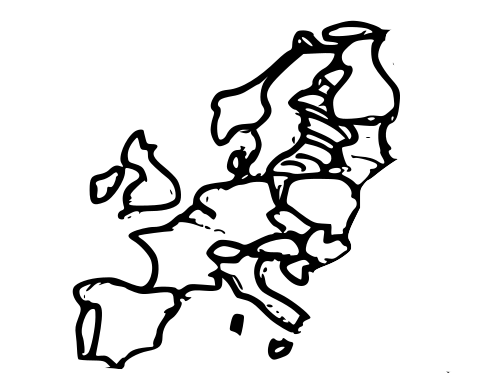
\includegraphics[width=1.5\textwidth]{imgs/europe.png}};
            %
            \draw[<-,ultra thick] ($(europe)+(-0.2,-0.7)$) .. controls ($(europe)+(-4,-0.7)$) .. ($(europe)+(-5,-0.9)$) node [below left,align=center,font=\scriptsize] {\emphcolor{Brown}{\textbf{Inria / Insa / Ensai / CentraleSupélec}}~\\ \emphcolor{Brown}{T. Guyard, C. Herzet, C. Elvira, A. Arslan}~\\\textit{\emphcolor{Brown}{Generalization, acceleration}}};
        }
        %
        %
        %
        \onslide<+-> {
            \draw[<-,ultra thick] ($(europe)+(0.7,1)$) .. controls ($(europe)+(0.5,1.5)$) .. ($(europe)+(1.1,3.5)$) node [above,align=center,font=\scriptsize] {\textbf{Lund University}~\\ M. Carlsson, C. Olsson...~\\\textit{Quadratic envelope}};
            %
            \draw[<-,ultra thick] ($(europe)+(0.4,0.1)$) .. controls ($(europe)+(-0.5,1.5)$) .. ($(europe)+(-1.2,2.5)$) node [above,align=center,font=\scriptsize] {\textbf{Frankfurt / Wurzburg Universities}~\\ C. Kanzow, A. Tillmann, ...~\\\textit{Optimality conditions}};
            %
            \draw[<-,ultra thick] ($(europe)+(-0.4,0.5)$) .. controls ($(europe)+(-1,1.3)$) .. ($(europe)+(-2,1.5)$) node [above left,align=center,font=\scriptsize] {\textbf{London Business School}~\\ J. Pauphilet, R. Cory-Wright, ...~\\\textit{Healthcare applications}};
            %
            \draw[<-,ultra thick] ($(europe)+(0.2,-0.6)$) .. controls ($(europe)+(-1.5,0.8)$) .. ($(europe)+(-2.5,0.9)$) node [left,align=center,font=\scriptsize] {\textbf{Ponts ParisTech}~\\ M. De Lara, P. Chancelier, A. Parmentier, ...~\\\textit{Non-convex analysis for $\ell_0$-norm, ML appli.}};
            %
            \draw[<-,ultra thick] ($(europe)+(-0.4,-0.4)$) .. controls ($(europe)+(-1,-0.4)$) .. ($(europe)+(-5,-0.2)$) node [left,align=center,font=\scriptsize] {\textbf{Centrale Nantes / ENSTA Bretagne}~\\ S. Bourguignon, J. Ninin, ...~\\\textit{Branch-and-Bound for $\ell_0$-problems}};
            %
            \draw[<-,ultra thick] ($(europe)+(0,-0.9)$) .. controls ($(europe)+(-0.5,-1.5)$) .. ($(europe)+(-1.2,-1.5)$) node [left,align=center,font=\scriptsize] {\textbf{IRIT / I3S}~\\ E. Soubies, L. Blanc-Féraud, ...~\\\textit{Tight relax. of $\ell_0$-norm}};
        }
        %
        %
        %
        \onslide<+-> {
            %
            \node[align=center,text width=0.3\linewidth] (usa) at ($(current page.center)+(-2.3,1.7)$) {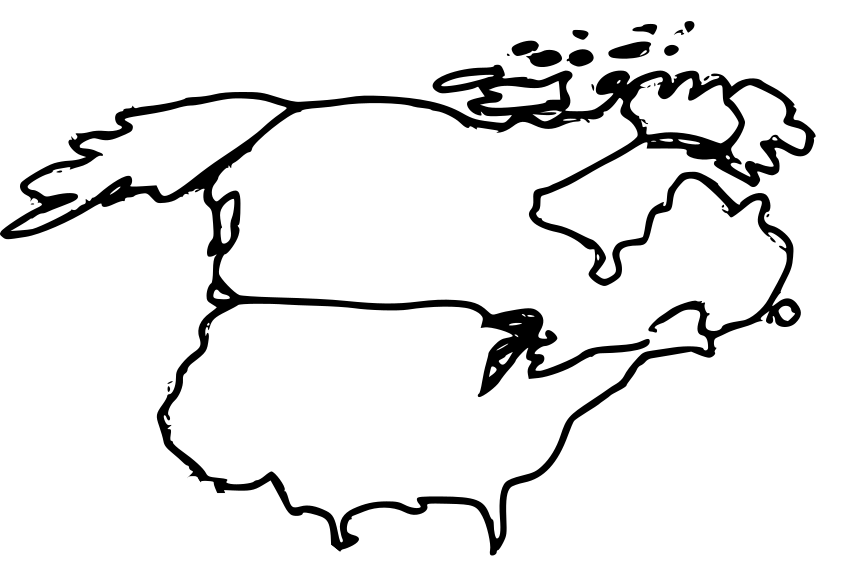
\includegraphics[width=1.5\textwidth]{imgs/usa.png}};
            %
            \draw[<-,ultra thick] ($(usa)+(1.9,-0.7)$) .. controls ($(usa)+(4.7,-0.4)$) .. ($(usa)+(5,0.3)$) node [above,align=center,font=\scriptsize] {\textbf{MIT}~\\ D. Bertsimas, R. Mazmuder, ...~\\\textit{MIO theory for $\ell_0$-problems}};
            %
            \draw[<-,ultra thick] ($(usa)+(0.25,0.45)$) .. controls ($(usa)+(-1.9,0.1)$) .. ($(usa)+(-2.3,-0.1)$) node [below,align=center,font=\scriptsize] {\textbf{Google Deep Mind}~\\ H. Hazimeh, A. Dedieu, ...~\\\textit{MIO-based heuristics}};
            %
            \draw[<-,ultra thick] ($(usa)+(-0.5,-1.2)$) .. controls ($(usa)+(-1.5,-1.4)$) .. ($(usa)+(-2,-1.9)$) node [below,align=center,font=\scriptsize] {\textbf{Berkley}~\\ A. Atamtürk, A. Gomès, ...~\\\textit{Convex-based acceleration}};
        }
    \end{tikzpicture}
\end{frame}
\begin{frame}{}
  \begin{tikzpicture}[remember picture,overlay]
    \node at ($(current page.north)+(0,-2)$) {\Large\textbf{\emphcolor{Brown}{Take-home message}}};
    \node[align=left,text width=1.1\textwidth] at ($(current page.north)+(0,-5.5)$) {
      \begin{itemize}
        \item[$\bullet$] \emphcolor{Brown}{$\ell_0$-norm problems} arise in many applied mathematical fields
        \item[$\bullet$] \emphcolor{Brown}{Mixed-integer optimization} tools to address them
        \item[$\bullet$] \emphcolor{Brown}{Structure exploitation} is the key to achieve competitive performances
        \item[$\bullet$] Active research area
        \begin{itemize}
          \item[$\rightarrow$] Theoretical results
          \item[$\rightarrow$] Efficiency, flexibility and accessibility of solution methods
          \item[$\rightarrow$] Software development
          \item[$\rightarrow$] Diffusion to other communities
        \end{itemize}
      \end{itemize}
    };
  \end{tikzpicture}
\end{frame}
\begin{frame}[standout]
    \begin{tikzpicture}[remember picture,overlay]
        \node[align=center] at ($(current page.center)+(0,-0)$) {Question time \\~\\ 
\includegraphics[width=30pt]{imgs/nerd_face.png}};
        % \node at ($(current page.north)+(0,-5)$) {
        %     
\includegraphics[width=30pt]{imgs/nerd_face.png}
        % };  
    \end{tikzpicture}
\end{frame}


\end{document}